\chapter{Variables biofísicas}
El objetivo de esta clase es obtener, de distintas maneras, variables biofísicas utilizando imágenes satelitales. Para hacerlo se utilizarán dos tipos de modelos:

\begin{itemize}
    \item Semi-empiricos: obtenidos a partir de datos de campo.
    \item Multiespectrales: obtenidos utilizando el \emph{Biophysical processor} del SNAP.
\end{itemize}

\section{Diagramas de dispersión}

Abra la imágen \path{S2A_MSIL2A_20170720.dim} que se encuentra en la carpeta \path{material/raster_data}.

Una herramienta util para explorer el comportamiento de la capa raster es observar los distintos cortes del espacio espectral. Para ello habra la herramienta \emph{Analysis/Scatter plot} (Figura \ref{fig:scatter}).

\begin{figure}[h!]
    \centering
    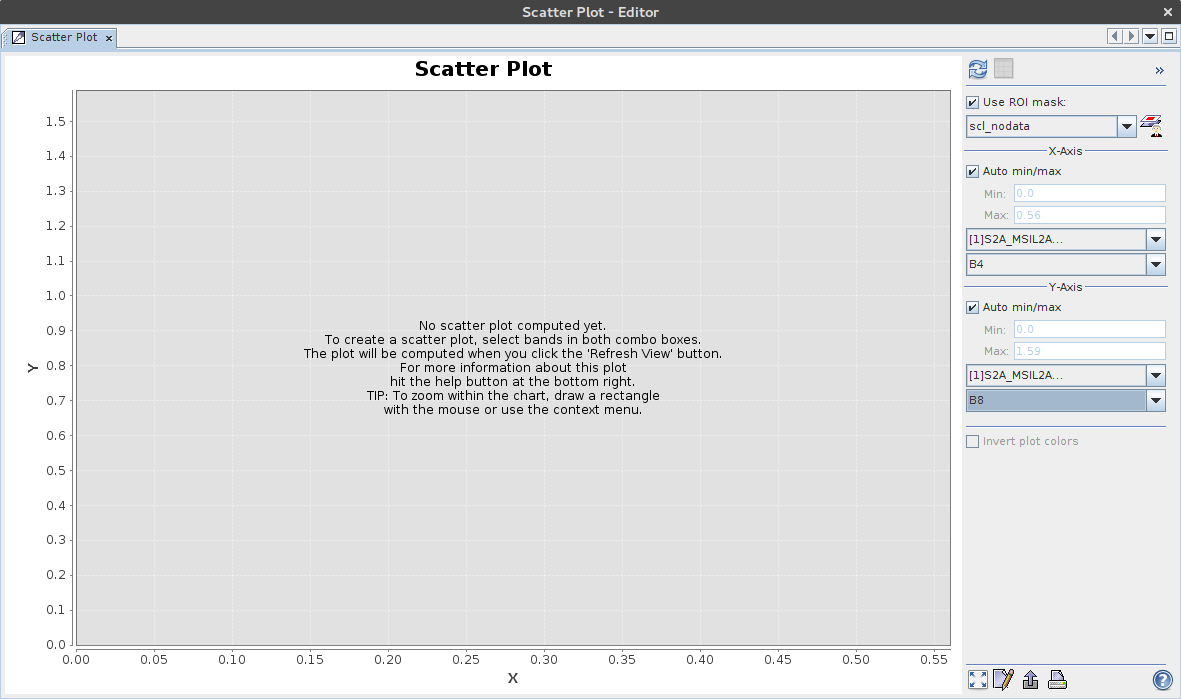
\includegraphics{fig:scatter.png}
    \caption{}
    \label{fig:scatter}
\end{figure}

Seleccione la imagen y banda que corresponde a cada eje. Use en este caso la banda 4 (B4 - correspondiente a la region del rojo) y la banda 8 (B8 - correspodiente a la region del infrarrojo cercano) y haga click en el boton \emph{Refresh}.

Es posible cambiar los minimos y máximos para cada una de las bandas o dejar que el SNAP los configure automaticamente. Luego de cada cambio deberá presionar el boton refresh. Configure los valores para observar mejor el scatterplot.

Es posible también mostrar el scatterplot para una sola región de la imagen. Puede hacer esto seleccionando la opción \emph{Use ROI mask} y luego la mascara correspodiente. Utilice las máscaras

\begin{itemize}
    \item scl\_vegetation
    \item scl\_bare\_soil\_desert
    \item scl\_water
\end{itemize}

para comparar que regiones del scatterplot corresponden a cada tipo de cobertura (Figura \ref{fig:scatterVSW}).

\begin{figure}[h!]
    \centering
    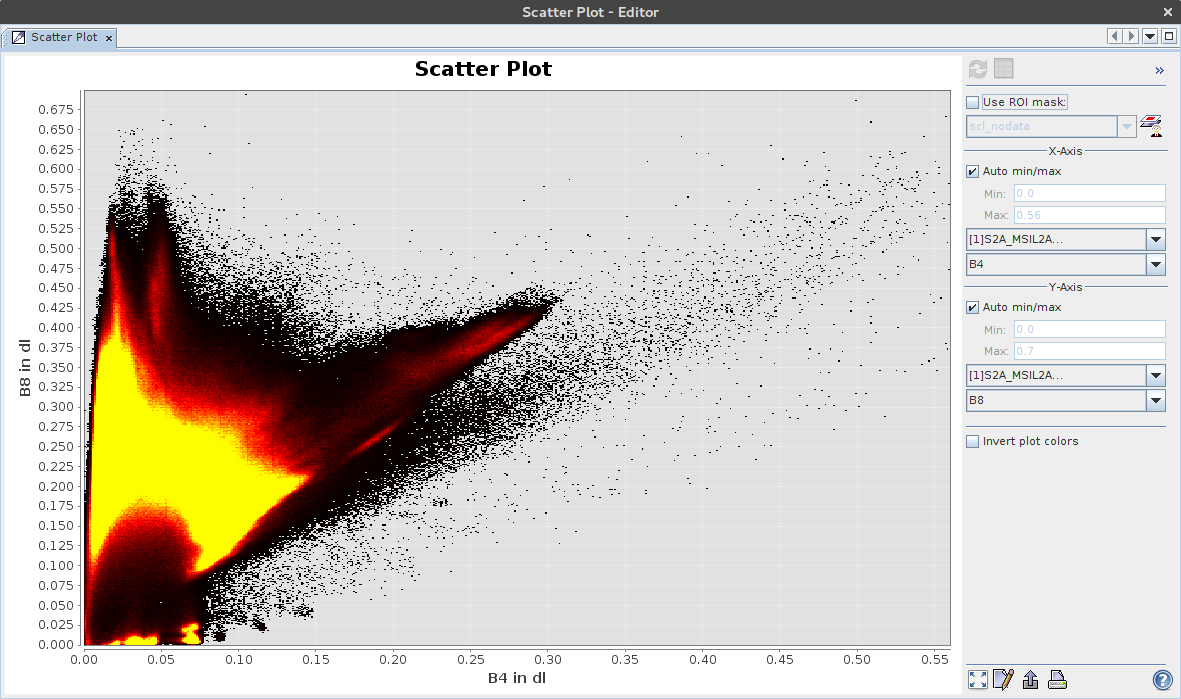
\includegraphics{fig:scatterVSW.png}
    \caption{}
    \label{fig:scatterVSW}
\end{figure}

Muevase en el scatterplot a la región correspodiente al agua y cambie los limites de los ejes para centrarse en dicha region. Haciendo click derecho sobre el gráfico seleccione la opción \emph{Select Mask 'scatter\_plot\_area'} y seleccione los daatos correspondientes a los pixeles con reflectancia en rojo de 0.07 y en nir de 0.005. (Figura \ref{fig:scatterwater}).

\begin{figure}[h!]
    \centering
    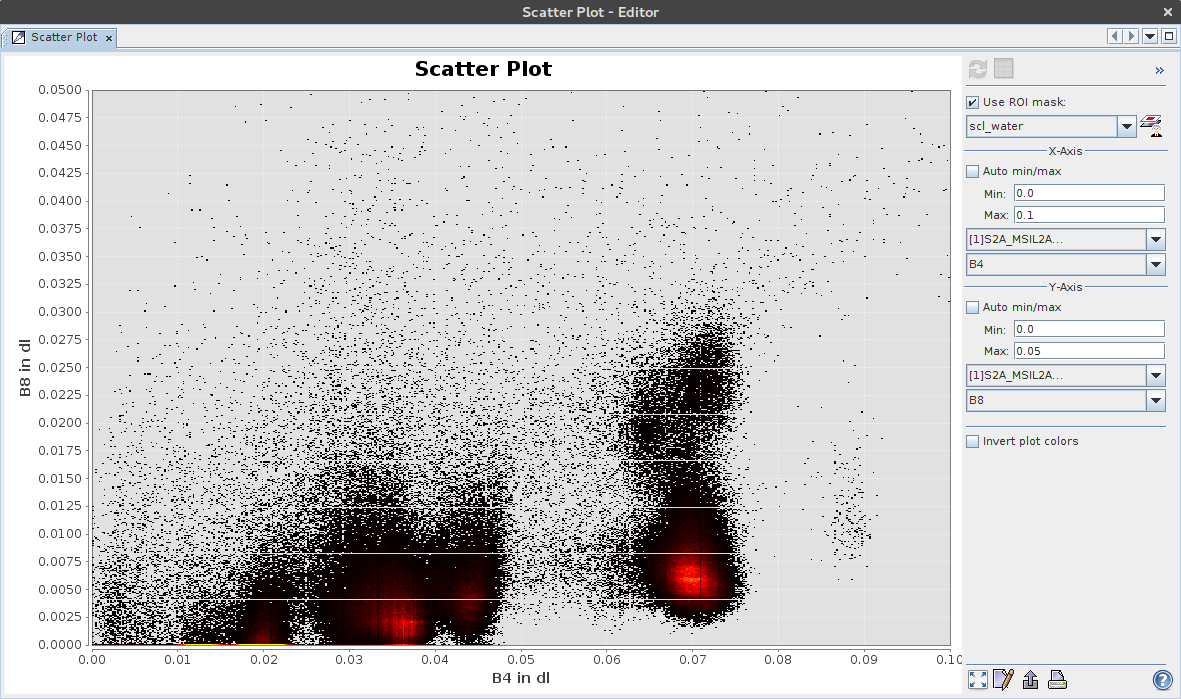
\includegraphics{fig:scatterwater}
    \caption{}
    \label{fig:scatterwater}
\end{figure}

Observe en la imagen cuales son los pixeles enmascarados y  que cobertura pertenecen.

\begin{que}
    ¿Puede distinguir en el scatterplot red-nir los distintos tipos de coberturas de agua? ¿Cual de las dos bandas le permite distinguirlos mejor? ¿Que pasa con las coberturas de vegetacion? ¿Es posible distinguir en este scatterplot las coberturas de selva y forestacion?  ¿Y con las de suelo desnudo? ¿Es posible distinguir en este scatterplot las zonas correspondientes a areas urbanas y con suelo desnudo? ¿Como interpreta la linea por debajo de la cual no hay valores? ¿A que cobertura pertenece?
\end{que}

\section{Cálculo de índices}

Existen distintos índices de vegetación que puede calcular utilizando el SNAP. En el menú \emph{Optical/Thematic Land processing/Vegetation Radiometric Indices} puede encontrar distintos indices de vegetación. Seleccione el NDVI de la lista y calculelo para la imagen. Deberá elegir en la sección de \emph{Processing parameters} las bandas a utilizar. Elija la banda 4 y 8 para los parametros red y nir respectivamente (Figura \ref{fig:ndviconfig}). El proceso tomara unos segundos y creará un nuevo archivo con los indices de vegetacion.

\begin{figure}[h!]
    \centering
    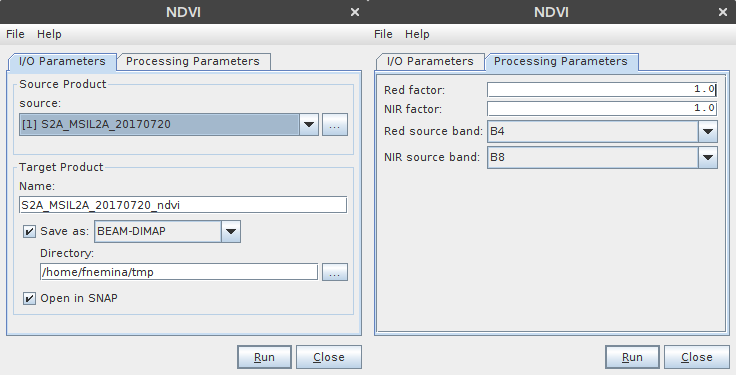
\includegraphics[scale=1.2]{fig:ndviconfig.png}
    \caption{}
    \label{fig:ndviconfig}
\end{figure}

Muestre el NDVI generado. Puede cambiar los colores y la parte del histograma en la que se muestra la imagen desde la pestaña \emph{Colour managment} (Figura \ref{fig:cman}). Es posible además guardar y cargar paletass externas. Utilice en este caso la paleta \path{ndvi.cpd} que se encuentra en la carpeta \path{material/aux_data} para mostrar el NDVI haciendo click en \emph{Import colour palette from text file}.

\begin{figure}[h!]
    \centering
    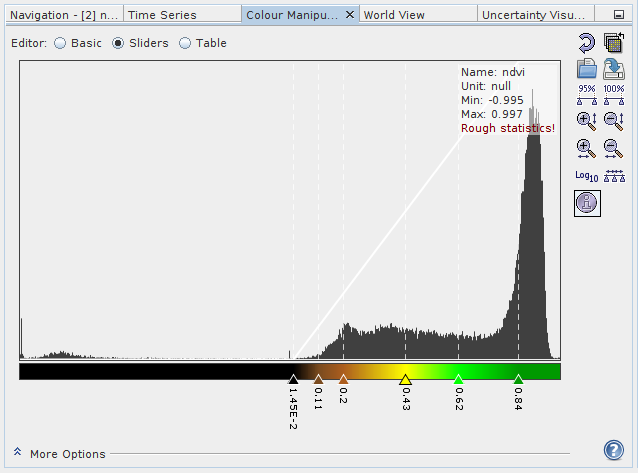
\includegraphics[scale=1.2]{fig:cman.png}
    \caption{}
    \label{fig:cman}
\end{figure}

Calcule el SAVI para la misma imagen (Figura \ref{fig:saviconfig}). comparelo con el NDVI. Puede ver ambas imagenes en simultaneo haciendo click en \emph{Windows/Tile horizontaly} o \emph{Windows/Tile vertically}. Para volver a la vista de una sola imagen haga click en \emph{Windows/Tile single}.


\begin{figure}[h!]
    \centering
    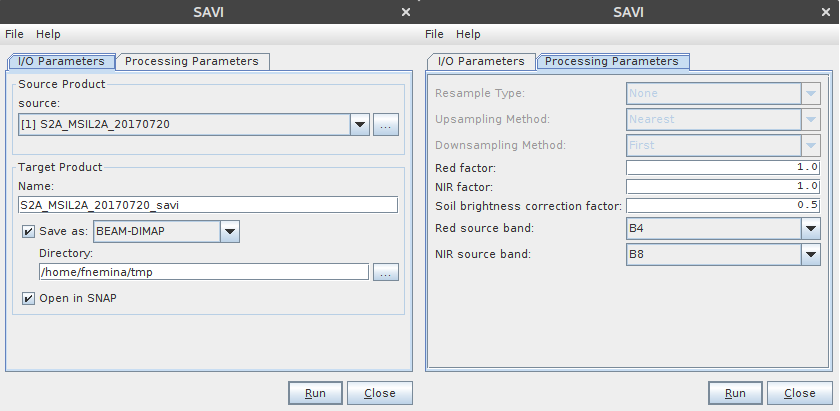
\includegraphics[scale=1.2]{fig:saviconfig.png}
    \caption{}
    \label{fig:saviconfig}
\end{figure}

Finalmente, construya el scatterplot entre el NDVI y el SAVI. Deberá en este caso seleccionar 2 imágenes distintas como fuente. Restrinja ademas el NDVI a los valores mayores que 0 (Figura \ref{fig:ndviscat}).

\begin{figure}[h!]
    \centering
    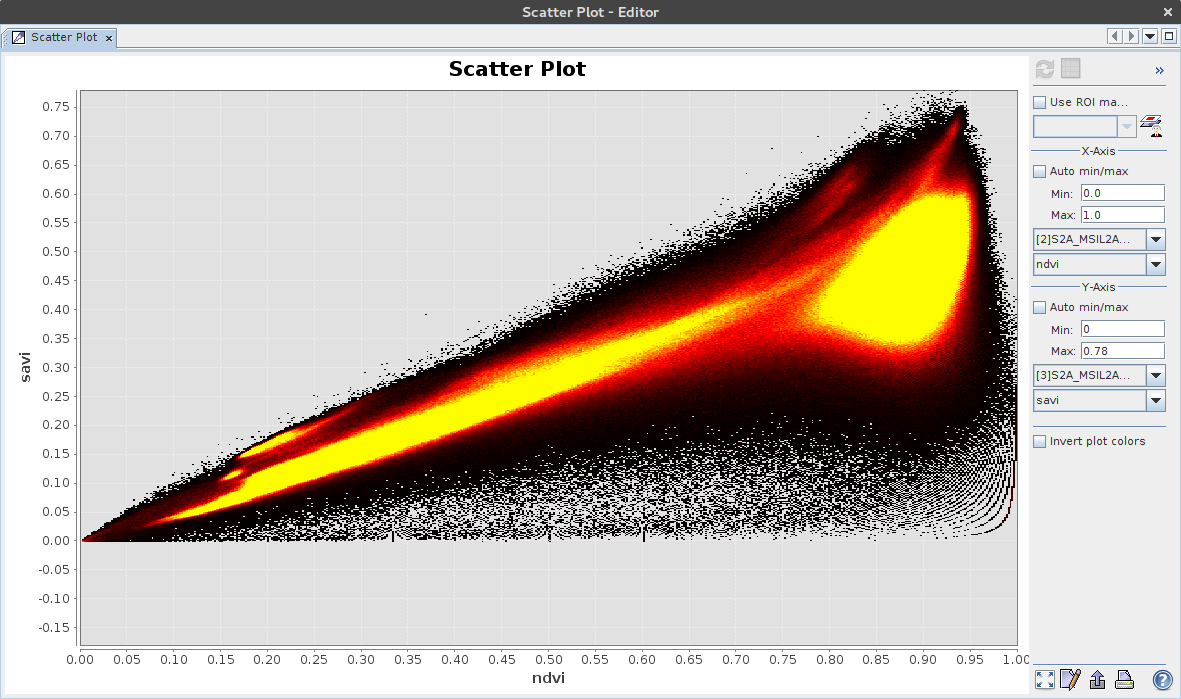
\includegraphics{fig:ndviscat.png}
    \caption{}
    \label{fig:ndviscat}
\end{figure}

\begin{que}
    ¿En que regiones es más alto el NDVI? ¿En que regiones es más bajo? ¿Coinciden estas regiones para el SAVI? ¿Cual de los dos índices le permite distinguir mayor variabilidad en las coberturas? ¿Que le dice esto sobre la saturación de los índices? ¿Por debajo de que valores el NDVI y el SAVI se comportan linealmente? ¿Por arriba de que valores dejan de hacer? ¿Que le dice esto sobre la saturación del SAVI comparada con el NDVI?
\end{que}

\section{Modelos de inversión}

Para construir los dinstintos tipos de modelo será de utilidad incorporar datos de campo con los que comparar. Para hacerlo seleccione la imagen \path{S2A_MSIL2A_20170720} del \emph{Product Explorer} y luego haga click en la herramienta \emph{Vector/Import/Vector from CSV}. Seleccione el archivo \path{mediciones.csv} de la carpeta \path{material/vector_data}. Se abrirá una nueva ventana que le pedirá el sistema de referencia (Figura \ref{fig:importV}) y luego otra que le pedira como interpretar los puntos importantes (Figura \ref{fig:importVI}).

\begin{figure}[h!]
    \centering
    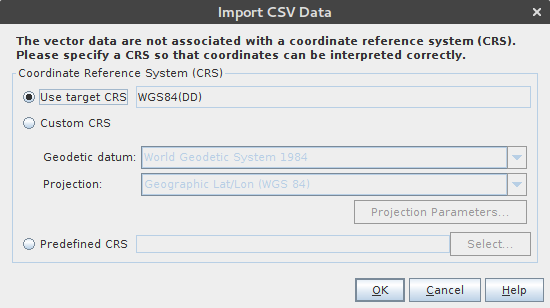
\includegraphics[scale=1.2]{fig:importV.png}
    \caption{}
    \label{fig:importV}
\end{figure}

\begin{figure}[h!]
    \centering
    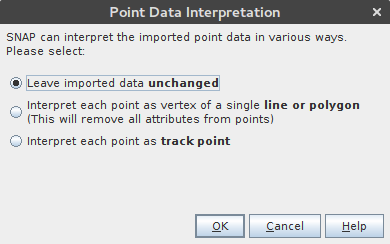
\includegraphics[scale=1.2]{fig:importVI.png}
    \caption{}
    \label{fig:importVI}
\end{figure}

Mantenga en ambas las opciones por defecto haciendo click en \emph{Ok}.

Puede explorar los contenidos del vector haciendo click en el vector \emph{Mediciones} dentor de \emph{Vector\_data} en el product explorer.

Incorpore estos datos a las imágenes creadas para el NDVI y el SAVI como lo hizo para la imagen multiespectral.

\subsection{Modelos semi-empiricos}

La herramienta \emph{Analysys/Correlative Plot} permite hacer gráficos entre los valores de un vector de tipo punto y los correspondientes valores en una imagen. Seleccione la banda \emph{ndvi} del NDVI en el arbol de capas y abrá la herramienta. Luego elija el \emph{Poing data source} como \emph{Mediciones} y el \emph{data field} como \emph{Lai mean}. (Figura \ref{fig:corndvi})

\begin{figure}[h!]
    \centering
    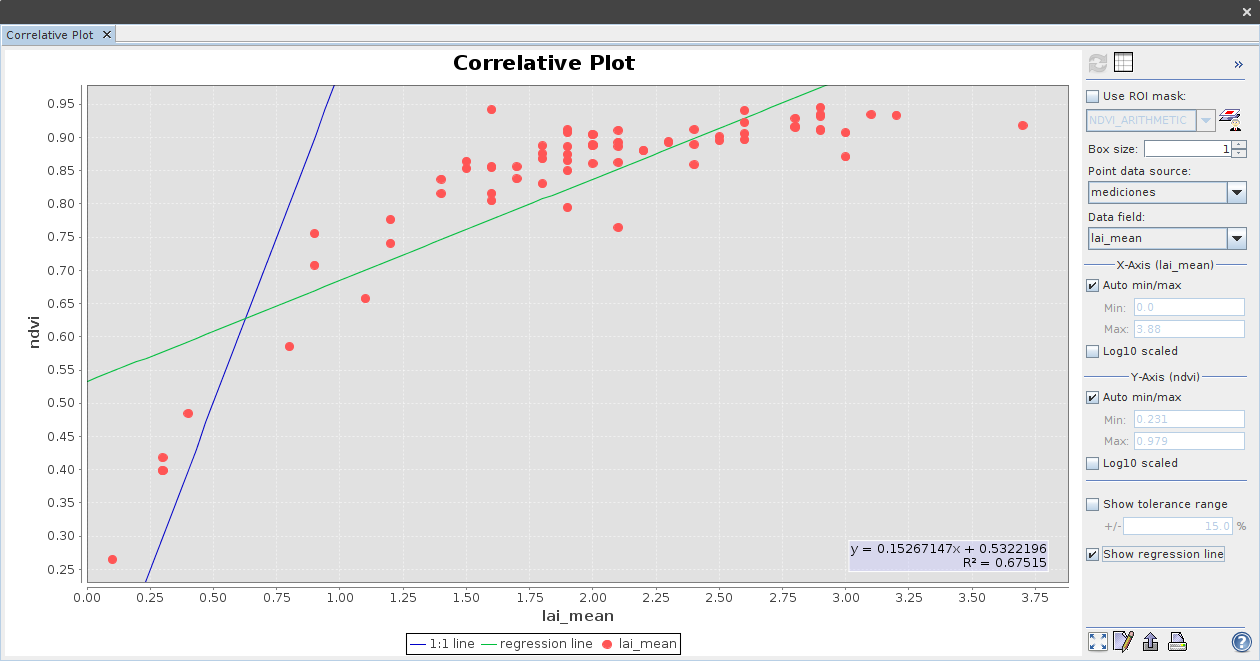
\includegraphics{fig:corndvi.png}
    \caption{}
    \label{fig:corndvi}
\end{figure}

Verá en este caso la linea 1:1 junto con los puntos medidos (en el eje horizontal) y los puntos de la imagen (en el eje vertical).

Agregue marcando la casilla \emph{Show regression line} la linea de tendencia y obtenga el valor que relaciona el NDVI con el LAI. Repita el proceso utilizando ahora la imagen correspondiente al SAVI.

Es posible utilizar este modelo sencillo para calcular un mapa de LAI. Para ello hacemos click derecho sobre la banda de NDVI y seleccionamos la opción \emph{Band maths...} (Figura \ref{fig:bm})

\begin{figure}[h!]
    \centering
    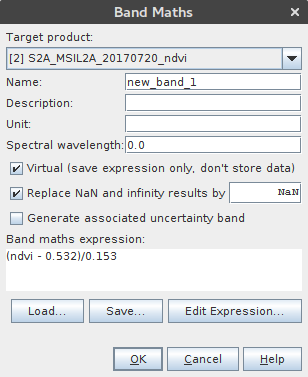
\includegraphics{fig:bm.png}
    \caption{}
    \label{fig:bm}
\end{figure}

Recuerde que la relación aquí obtenida es
\begin{equation}
    \nu = m \times \beta + b
\end{equation}
donde $\nu$ es el índice de vegetación y $\beta$ alguna variable biofísica. Por lo tanto la ecuación que debemos utilizar es
\begin{equation}
    \beta = \frac{\nu - b}{m}
\end{equation}

Utilice la ecuación

\begin{verbatim}
    (ndvi - 0.532)/0.153
\end{verbatim}

y ponga como nombre a la banda \emph{LAI}. Repita el proceso para el SAVI.

Compare utilizando la herramienta \emph{Correlative plot} el resultado del modelo obtenido con los datos medidos a campo.

\begin{que}
    ¿Cual de los dos índices se comporta de forma más lineal con el LAI? ¿Que pasa para el NDVI a medida que el LAI aumenta? ¿En que zona es lineal el NDVI y el LAI? ¿En que zona es lineal el SAVI y el LAI? ¿Cual de los dos modélos ajusta mejor a los datos a campo?
\end{que}

\subsection{Modelos multiespectrales}

Otra opción para calcular parametros biofísicos, en el caso de SENTINEL 2, es utilizar el \emph{Biophysical processor}. Este algorítmo considera en simultaneo todas las bandas de la imagen y medienta un modelo de inversión, obtiene los parametros biofísicos para la imagen.

Para utilizarlo elija la herramienta en \emph{Optical/Thematic Land processing/Vegetation Radiometric Indices}. Seleccione la imagen \path{S2A_MSIL2A_20170720} y elija computar el LAI (Figura \ref{fig:bio}). Haga click en \emph{Run} para ejecutar el modelo.

\begin{figure}[h!]
    \centering
    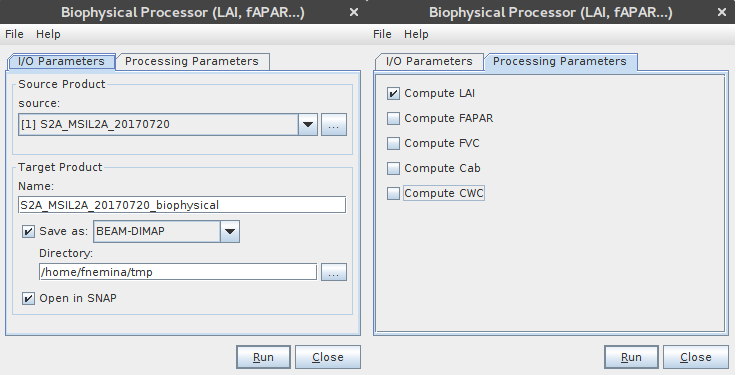
\includegraphics[scale=1.2]{fig:bio.png}
    \caption{}
    \label{fig:bio}
\end{figure}

\textbf{Importante:} Este proceso puede tomar entre algunos minutos y varias horas según el tamaño de la imagen y la computadora utilizada.

Compare los resultados medidos a campo con los obtenidos aplicando el procesador incluido en el SNAP \footnote{En este caso, el coeficiente de correlación será artificialmente alto. Los valores obtenidos a campo utilizados en el curso fueron obtenidos utilizando el \emph{Biophysical processor} e incorporandoles ruido gaussiano.}.

Por último, es posible comparar los resultados obtenidos para el LAI por los distintos métodos. Una forma de hacer esto es utilizar la herramienta \emph{Band maths...} para calcular la diferencia entre el LAI calculado por cada uno. En este caso utilice la opción \emph{Edit expression...} para poder utilizar bandas de distintas imágenes. Luego de hacer este proceso, utilice la herramienta de estadistica en \emph{Analysis/Statistics} para calcular los parametros de la imagen y el histograma (Figura \ref{fig:sta}).

\begin{figure}[h!]
    \centering
    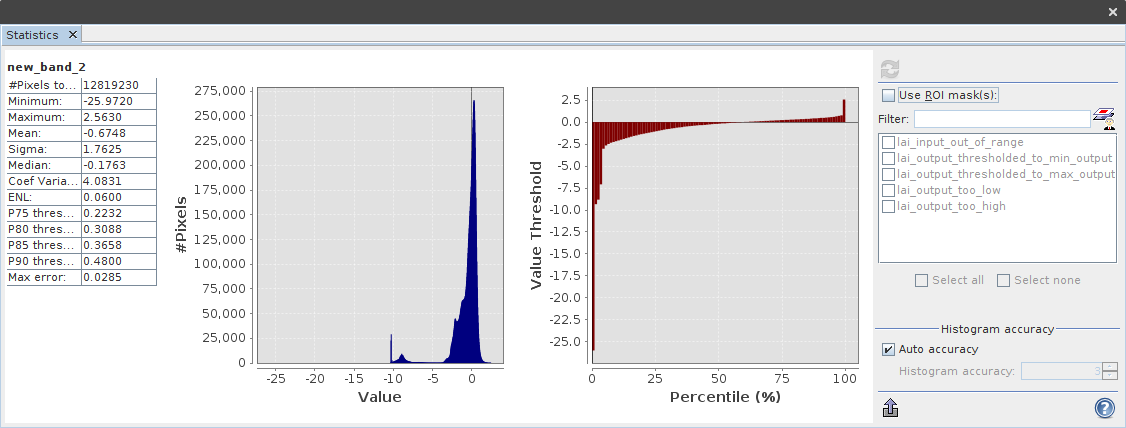
\includegraphics{fig:sta.png}
    \caption{}
    \label{fig:sta}
\end{figure}

\begin{que}
    ¿Cómo es el ajuste de los datos medidos a campo del procesador comparado con los índices? ¿Cual es la diferencia promedio entre el LAI calculado con cada uno de los índices y el del biophysical processor? ¿Cómo es el desvio? ¿Que modelos coincide?
\end{que}
